\documentclass{article}
% standard preamble reused across all online solves
\usepackage{graphicx}
\usepackage{float}
\usepackage{wrapfig}
\usepackage{caption}
\usepackage{subcaption}
\usepackage{booktabs}
\usepackage{array}
\usepackage{enumitem}
\usepackage[table]{xcolor}
\usepackage{amsmath, amssymb}
\usepackage{listings}
\usepackage{algorithm}
\usepackage{algpseudocode}
\usepackage{comment}
\usepackage[numbers]{natbib}
\usepackage{hyperref}
\usepackage{subcaption}
\usepackage{multirow}
\usepackage{amsthm}
\usepackage{minitoc}
\usepackage{authblk}

\title{Mathematical Foundations of Image Synthesis}
\author{Zarif Ishmam (2305035)}
\date{\today}


\begin{document}
\maketitle

\section{Introduction}
Image synthesis is the process of generating images from mathematical and algo
rithmic descriptions. Modern graphics systems rely on \textbf{precise mathematical models} and efficient computation. \textit{Even small numerical errors} can result in visible artifacts in rendered images.


Typical formulations involve scalar values such as $x$, indexed parameters
like $I_{ij}$, and exponential terms $e^{x^2}$. These elements are combined to simulate realistic lighting behavior.

\section{Core Components}
\subsection{Rendering Pipeline}
The rendering pipeline consists of the following stages:
% dash-labeled item mixed in with default bullets, then a nested itemize
\begin{itemize}
    \item Scene Definition 
    \item Camera Configuration
    \item[-] Light Placement \\
    
    \noindent\leftskip=-1cm{\textbf{Important} Shading Model}
        \begin{itemize}
            \item[-] Diffuse Shading
            \item[-] Specular Highlights
        \end{itemize}
\end{itemize}

\subsection{Execution Order}
% nested enumerate uses [(a)] to force lowercase-letter sub-labels
\begin{enumerate}
    \item Input Processing
    \item Ray Construction
        \begin{enumerate}
            % note: both items below use [(a)], the second [(a)] auto-advances to (b) in the pdf
            \item[(a)]Primary Rays
            \item[(a)] Secondary Rays
        \end{enumerate}
    \item  Intersection Evaluation
        \begin{itemize}
            \item Object Hit Test
        \end{itemize}
\end{enumerate}

\section{Mathematical Modeling}
Light interaction with surfaces can be expressed using the following equations.

% equation environment auto-numbers; $$...$$ is unnumbered display math
\begin{equation}
    L = I_{ij}.\cos (\theta) + R^2
\end{equation}

$$
k = \frac{ab}{cd}
$$

% split keeps a multi-line derivation under a single equation number
\begin{equation}
\begin{split}
    f(x) &= x^2 + 2x + 1 \\
    &= (x + 1)^2
\end{split}
\end{equation}

% cases environment for piecewise definitions
\[
f(x) = \begin{cases}
    y & \text{if } y \geq 0 \\
    -x  & \text{if } y < 0
\end{cases}
\]

\[
p(t) = \begin{cases}
    0,  t < 0 \\
    e^{-t}, 0 <= t < 3, \\
    \ln (t - 2), t >= 3
\end{cases}
\]

$$
\mathcal{N}(x_i, \mu, \sigma) = \frac{1}{\sqrt2\pi\sigma}e^{-\frac{x_i - \mu}{2\sigma ^2}}
$$

\section{Performance Comparison}

% multirow spans the "Ray Tracing" rows; multicolumn spans "Hybrid Method" across the first two columns
\begin{table}[H]
    \centering
    \begin{tabular}{|c|c|c|}
         \hline
         Method & Accuracy & Time Complexity  \\
         \hline
         Rasterization & Medium & $O(n)$ \\
         \hline
         \multirow{2}{*}{Ray Tracing} & High & $O(n^2)$ \\
        & Very High & $O(n^3)$ \\
        \hline
        \multicolumn{2}{|c|}{Hybrid Method} & $O(n^2)$ \\
        \hline
    \end{tabular}
    \caption{Comparison of Image Synthesis Techniques}
    \label{tab:t1}
\end{table}

The results in ~\ref{tab:t1}  highlight the trade-off between accuracy and computational cost.

\section{Visual Illustration}
% three subfigures placed side by side with \hfill spacing between them
\begin{figure}[H]
    \centering
    \begin{subfigure}{0.3\textwidth}
        \centering
        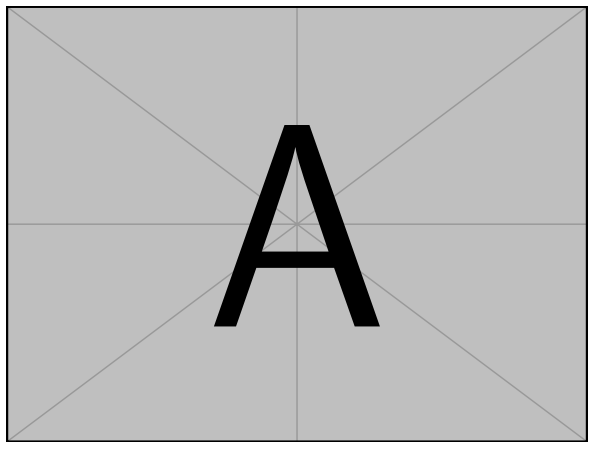
\includegraphics[width=\linewidth]{A.PNG}
        \caption{Output A}
    \end{subfigure}
    \hfill
    \begin{subfigure}{0.3\textwidth}
        \centering
        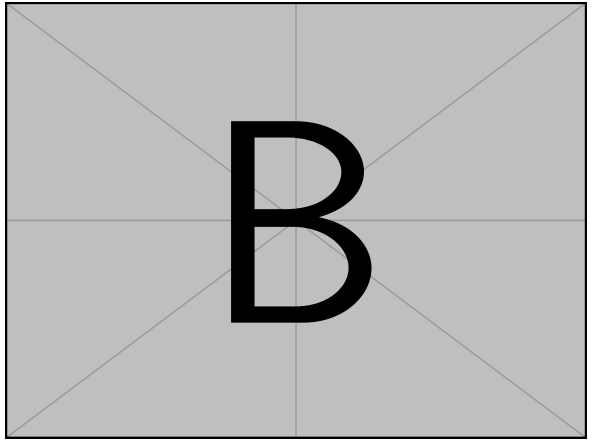
\includegraphics[width=\linewidth]{B.PNG}
        \caption{Output B}
    \end{subfigure}
    \hfill
    \begin{subfigure}{0.3\textwidth}
        \centering
        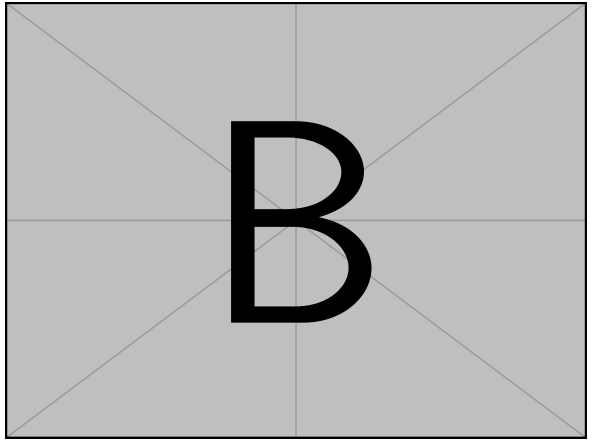
\includegraphics[width=\linewidth]{B.PNG}
        \caption{Output B}
    \end{subfigure}
    \caption{Caption}
    \label{fig:f1}
\end{figure}

Figure ~\ref{fig:f1} compares three different rendering outputs arranged in a single row.

\section{Conclusion}
Image synthesis combines \underline{mathematical precision}, algorithmic design, and effi
cient implementation. As scene complexity increases, choosing the appropriate
method becomes critical for balancing quality and performance.

\end{document}